\section{Results}
\subsection{Amsterdam Urban Tree Dataset}
Our analysis focused exclusively on tile 25BZ1 within the Amsterdam municipality. Within this tile, our model detected approximately 12,000 trees, substantially exceeding the 3,929 public trees recorded in the municipality database. The municipal dataset, which includes species information for all entries, therefore captures only about one-third of the trees present in the tile: highlighting the model’s ability to identify both public and private or otherwise unregistered trees. 

\begin{figure}[h!]
    \centering
    % Single image
    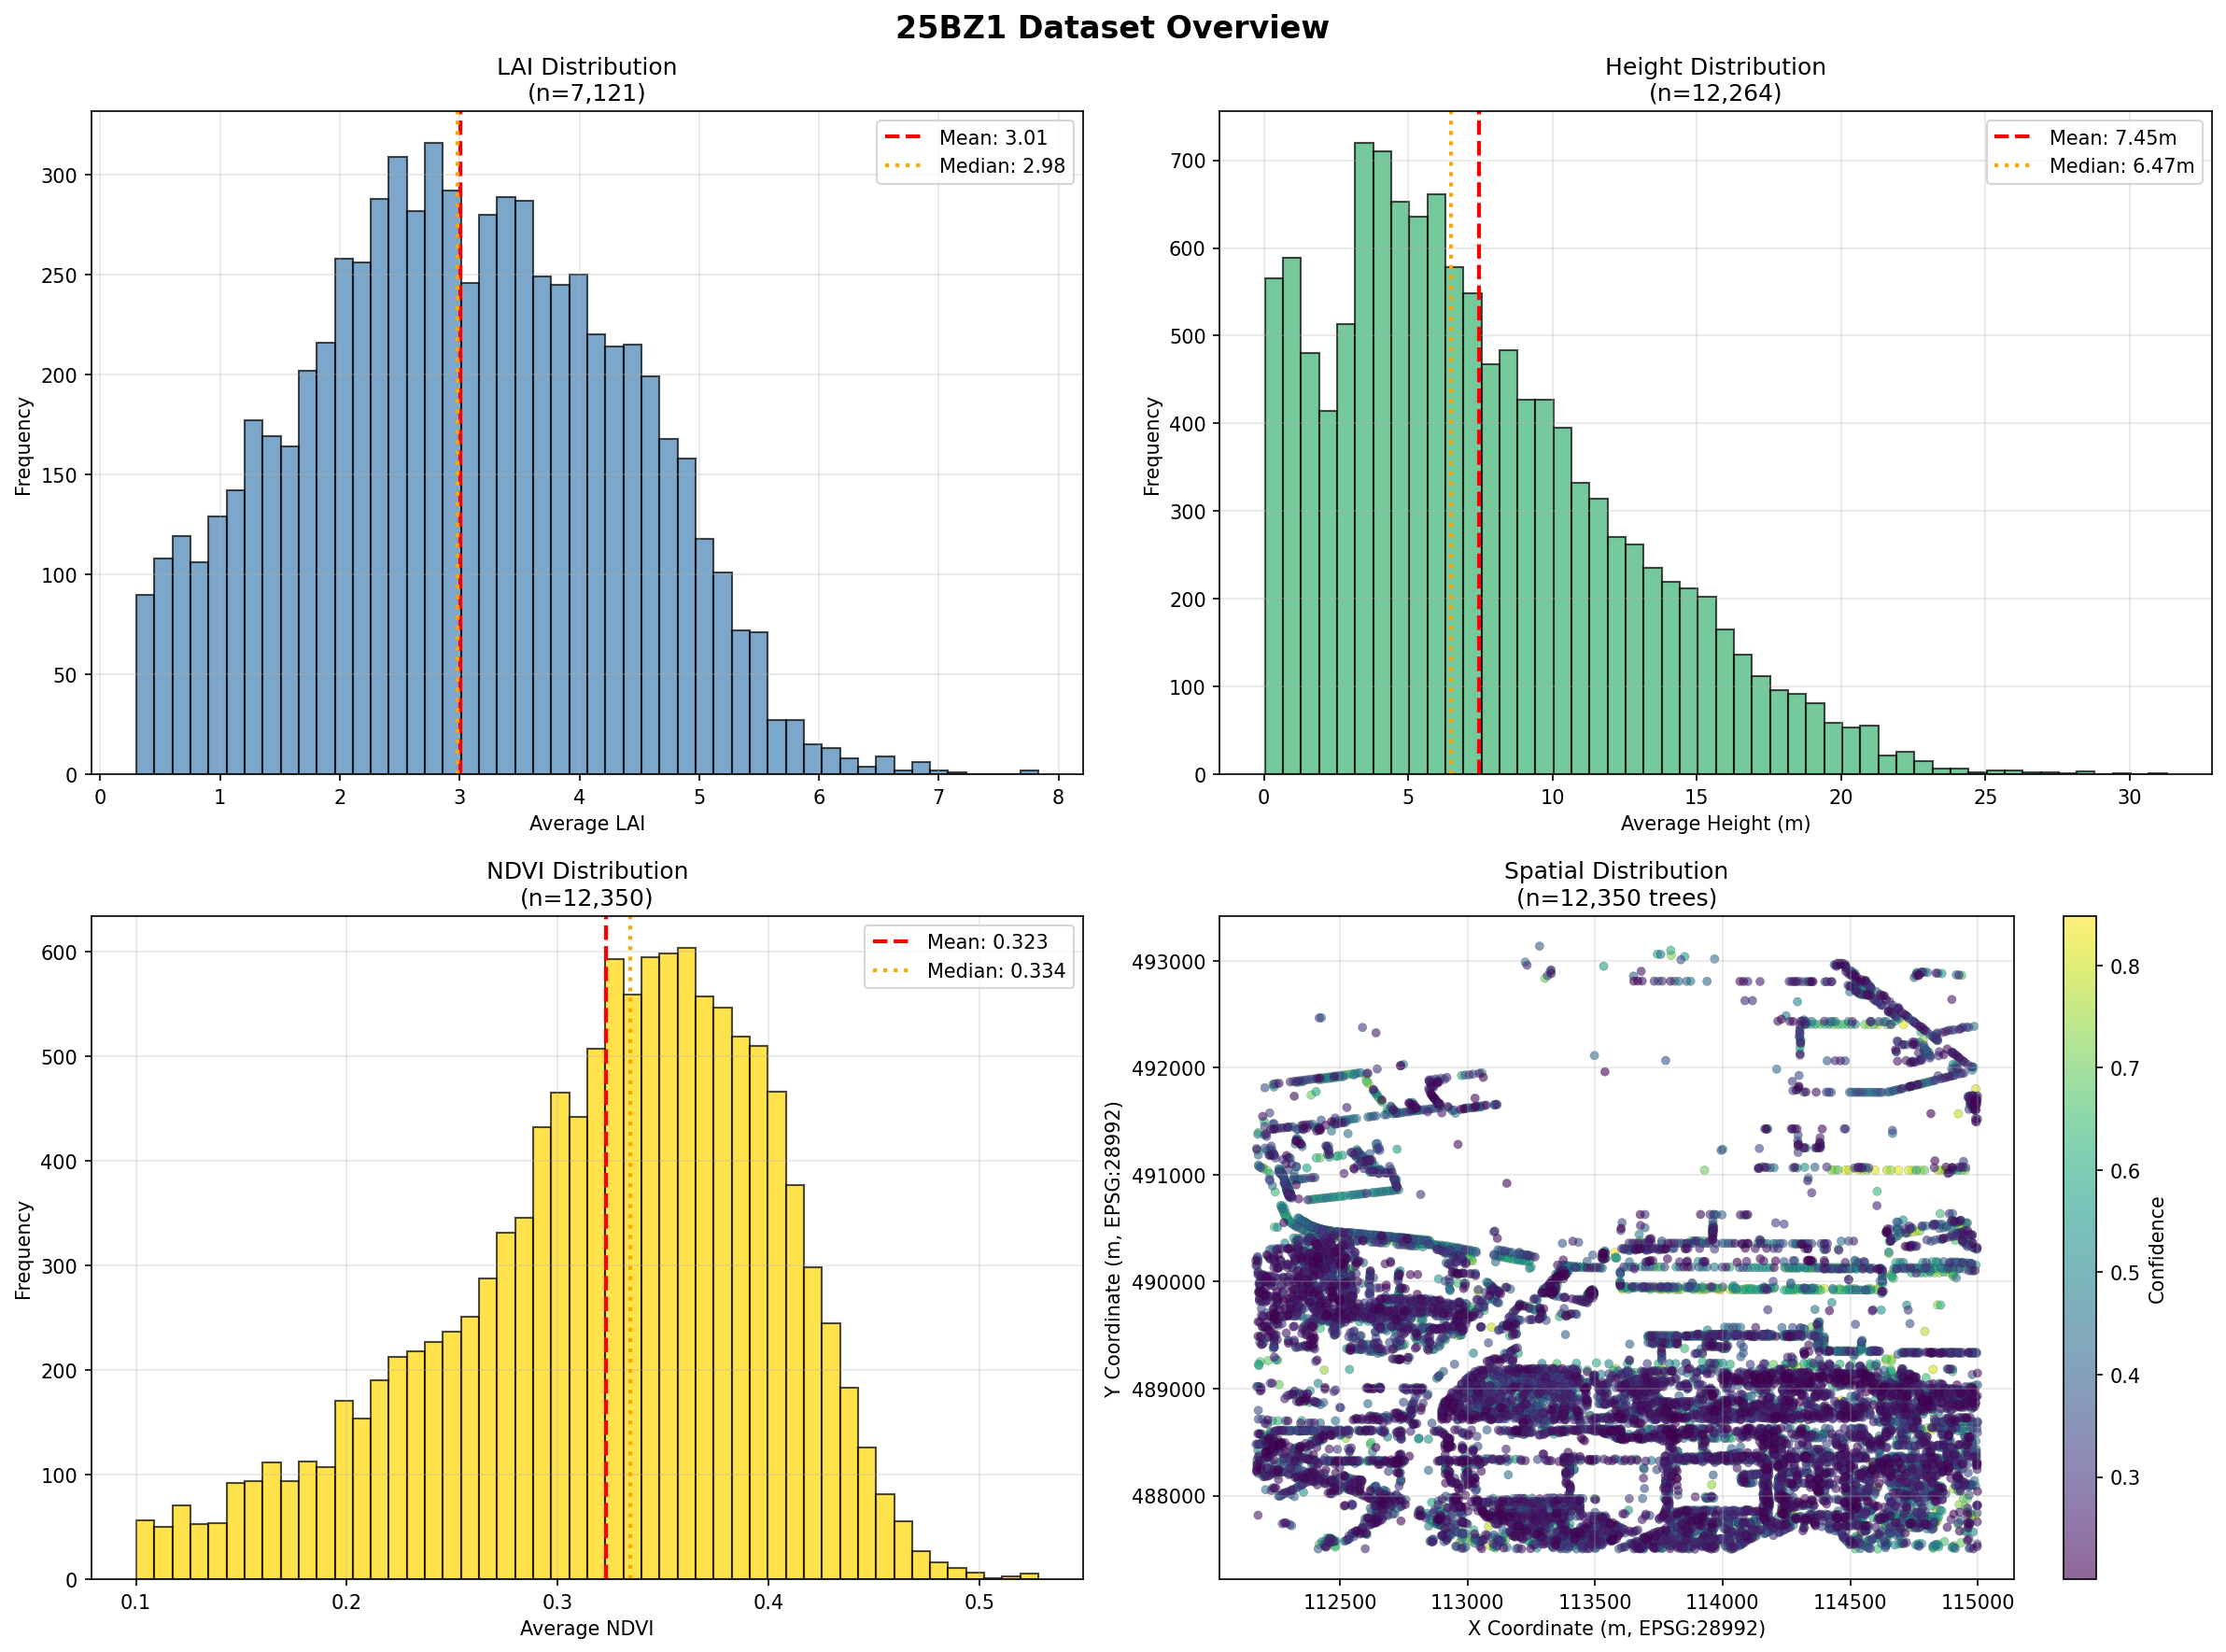
\includegraphics[width=\textwidth, height=\textheight, keepaspectratio]{figures/results/training/overview_multi_panel.png}
    \caption{Overview of our Tree Dataset}
    \label{fig:overview_dataset}
\end{figure}

The trees within tile 25BZ1 exhibited pronounced variability in their morphological and spectral properties. Leaf Area Index (LAI) ranged from $0.12$ to $8.45$ (mean $\pm$ SD: $3.21 \pm 1.33$), forming an approximately normal distribution with a slight right skew. Tree heights spanned $2.3$--$32.7$ m (mean: $12.4 \pm 5.8$ m), which aligns with typical urban forest structure---where median heights near $13$ m and ranges of $5$--$30$ m are expected \cite{rahmanTreeCoolingEffects2020}---apart from a small number of unusually low outliers. NDVI values ($0.21$--$0.89$; mean: $0.68 \pm 0.12$) indicated generally healthy canopy conditions. Among the 3,929 municipal trees, species distribution was dominated by Ulmus (N=287), Fraxinus (N=94), Acer (N=76), and Populus (N=52), supplemented by a large group of mixed or unidentified taxa (N=1,243).

The LAI values observed for the majority of trees (1–7) are consistent with previous investigations of urban canopies \cite{watts2018ReportLancet2018,faurieAssociationHighTemperature2022}, where LAI is typically lower than in natural forests. Species-specific distributions of height, NDVI, and LAI verify that proportions between species align with previous research (Supplementary Figure 2), with mean values matching expectations and top quantile variations reflecting urban factors such as tree age and municipal pruning practices \cite{kantorSmallscaleHumanbiometeorologicalImpacts2016}. 


%%% features relations


% \begin{figure}[h!]
%     \centering
%     % Single image
%     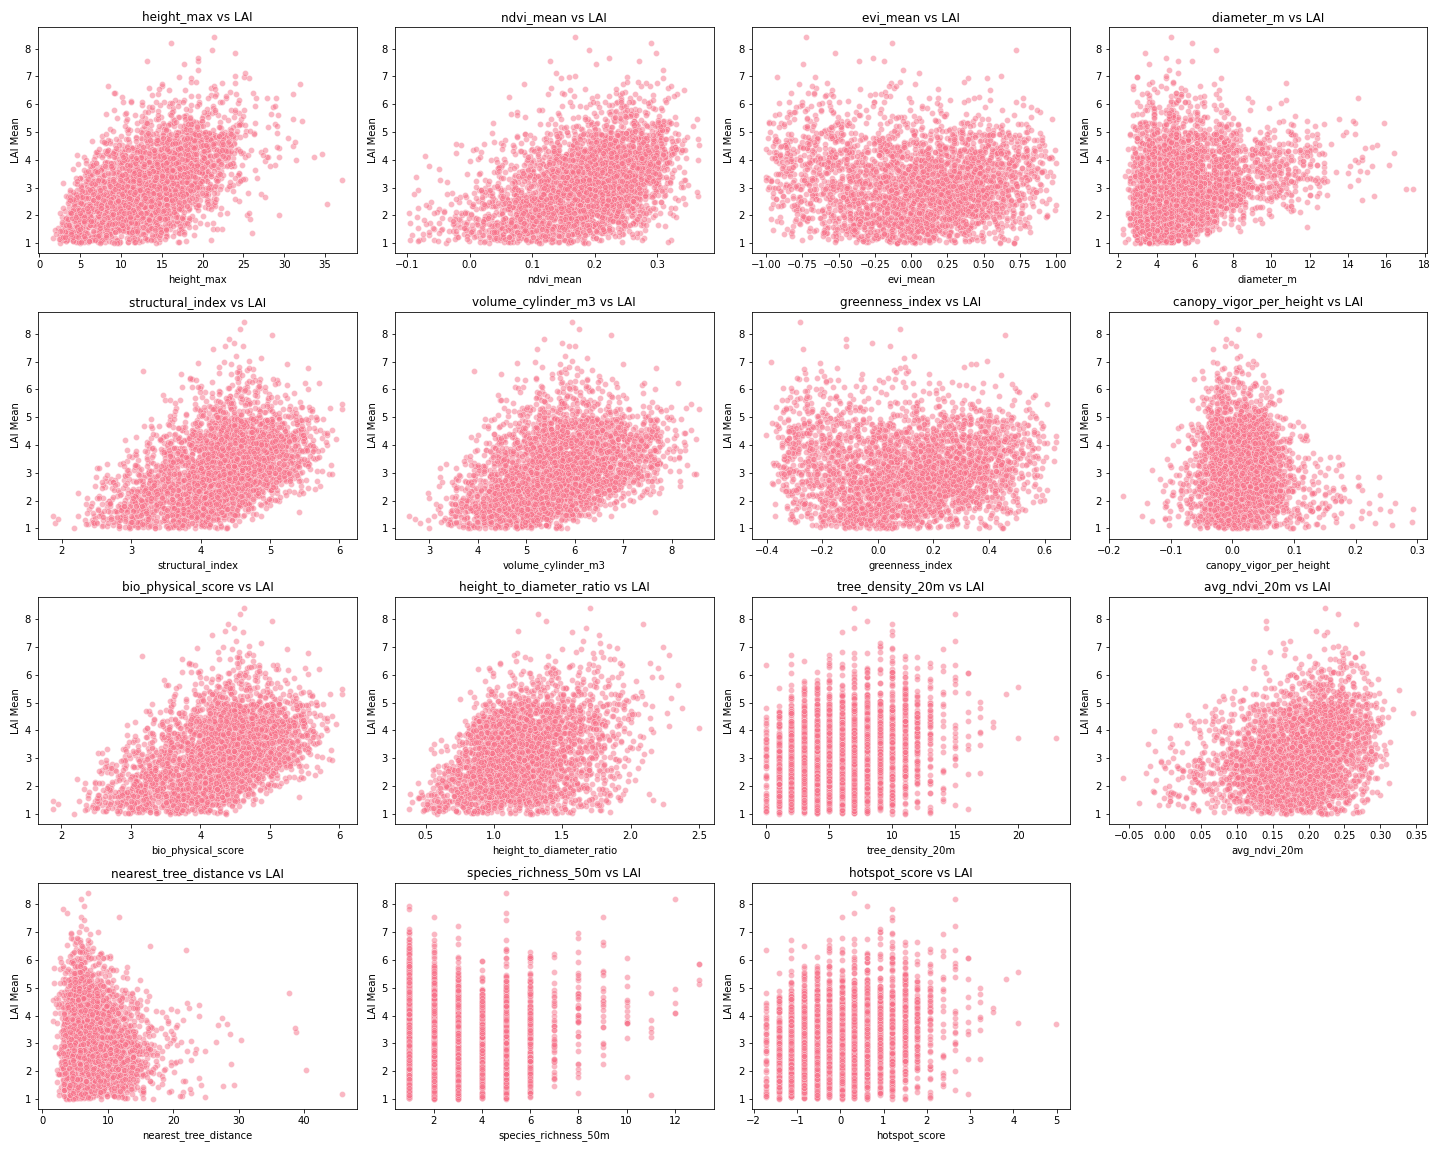
\includegraphics[width=0.3\textwidth, height=0.3\textheight, keepaspectratio]{figures/results/analytics/feature_vs_lai_scatter.png}
%     \caption{A single small image}
%     \label{fig:single_image}
% \end{figure}

%%Spatial Gradients Figures
% \begin{figure}[h!]
%     \centering
%     % First image
%     \begin{subfigure}[b]{0.3\textwidth} % Adjust width as needed for spacing
%         \centering
%         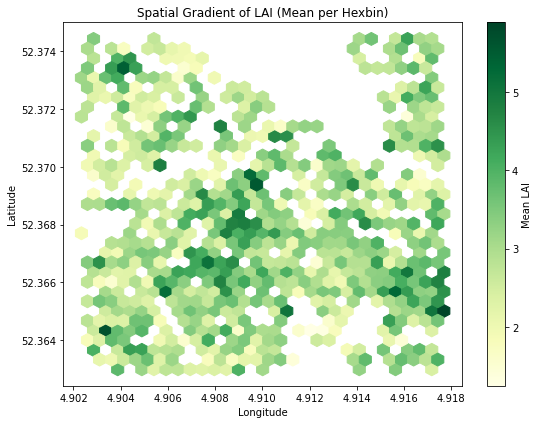
\includegraphics[width=\linewidth, height=\linewidth, keepaspectratio]{figures/results/analytics/lai_spatial_gradient_hexbin.png}
%         \caption{Caption for Image 1}
%         \label{fig:image1}
%     \end{subfigure}
%     \hfill % Adds horizontal space between subfigures
%     % Second image
%     \begin{subfigure}[b]{0.3\textwidth}
%         \centering
%         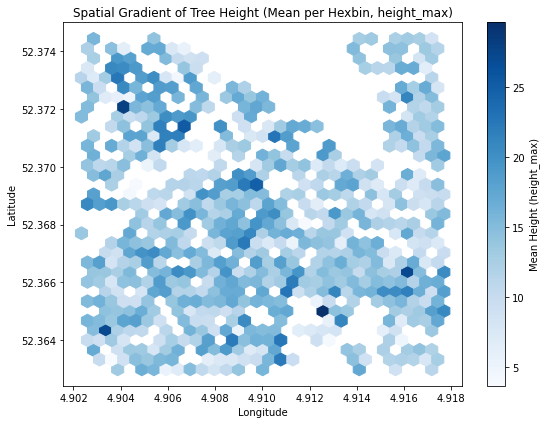
\includegraphics[width=\linewidth, height=\linewidth, keepaspectratio]{figures/results/analytics/height_spatial_gradient_hexbin_height_max.png}
%         \caption{Caption for Image 2}
%         \label{fig:image2}
%     \end{subfigure}
%     \hfill % Adds horizontal space between subfigures
%     % Third image
%     \begin{subfigure}[b]{0.3\textwidth}
%         \centering
%         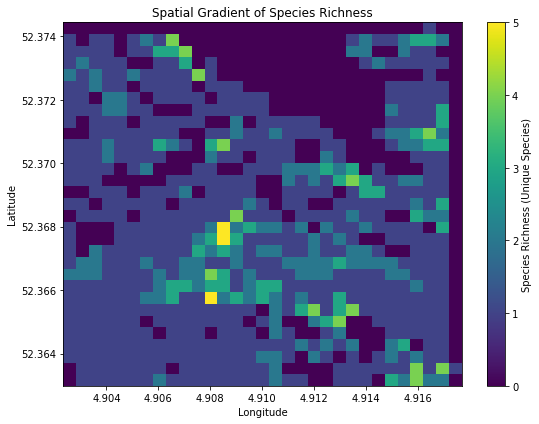
\includegraphics[width=\linewidth, height=\linewidth, keepaspectratio]{figures/results/analytics/species_richness_spatial_gradient_heatmap.png}
%         \caption{Caption for Image 3}
%         \label{fig:image3}
%     \end{subfigure}
%     \caption{Three images side-by-side}
%     \label{fig:three_images}
% \end{figure}


\subsection{LAI Prediction}



\subsubsection{Model Performance Comparison}

\begin{figure}[h!]
    \centering
    % Single image
    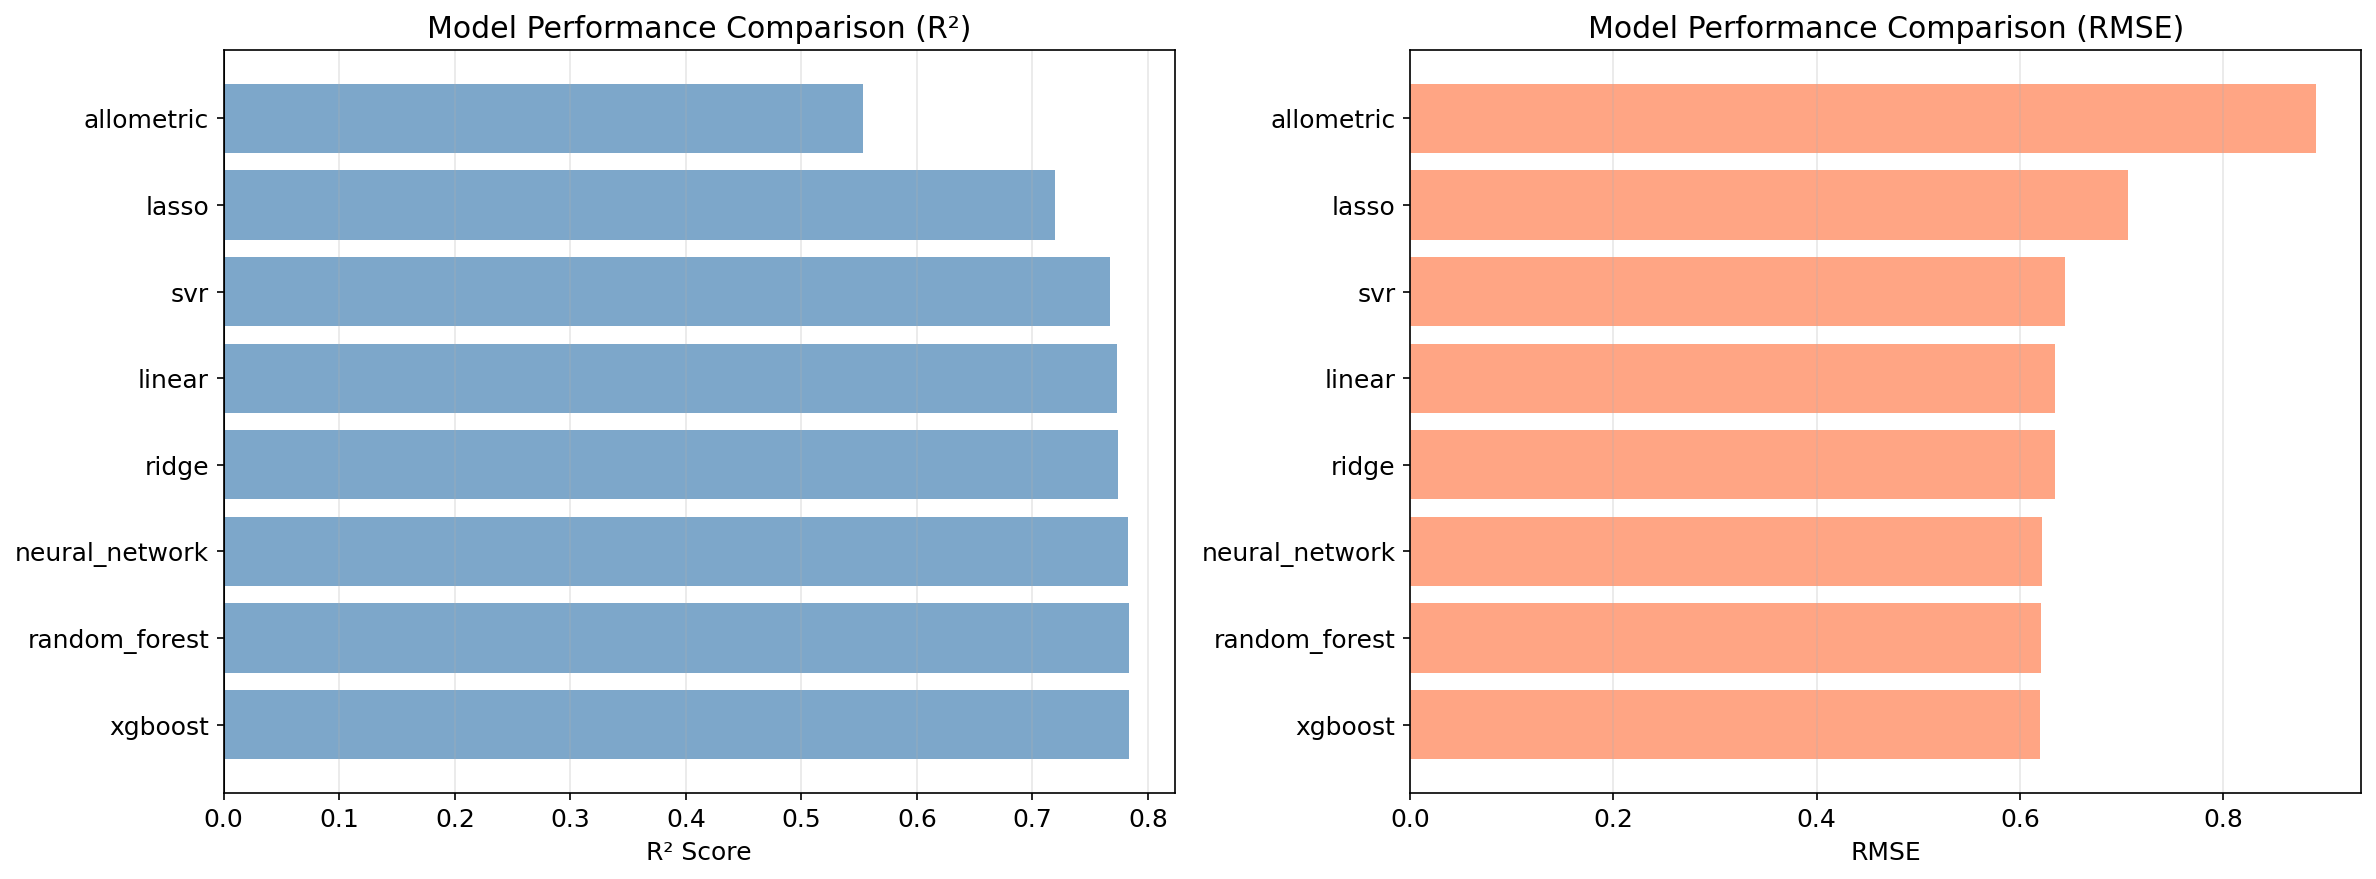
\includegraphics[width=\textwidth, height=\textheight, keepaspectratio]{figures/results/training/model_comparison.png}
    \caption{Comparative performance of LAI prediction models. XGBoost and Random Forest achieved highest accuracy (R² = 0.784), substantially outperforming traditional allometric baselines and linear models. Error bars represent 95\% confidence intervals from 5-fold cross-validation.}
    \label{fig:model_perf_comp}
\end{figure}

Eight predictive models were evaluated across multiple performance metrics (Table 1, Figure 2). Machine learning approaches substantially outperformed the traditional allometric baseline, with gradient boosting and ensemble methods achieving the highest predictive accuracy.

%%% TO ADD

Table 1. Comparative performance of LAI prediction models on the independent test set (N=1,063).

Note: Relative improvement calculated as: $$[(R^2_{model} - R^2_{allometric}) / R^2_{allometric}] × 100\%$$

XGBoost achieved the highest performance with a test $R^2$ of $0.784$ ($RMSE$ = $0.620$, $MAE$ = $0.462$), explaining $78.4\%$ of LAI variance and reducing prediction error by $30.4\%$ relative to the allometric baseline ($RMSE$ reduction from $0.891$ to $0.620$).
Random Forest performance was nearly identical ($R^2 = 0.784$, $RMSE = 0.620$, $MAE = 0.465$), while the neural network showed marginally lower performance ($R^2 = 0.783$).
Linear models with regularization (Ridge and Linear Regression) performed surprisingly well ($R^2 \approx 0.774$), suggesting that LAI relationships with morphological features are predominantly linear with modest benefit from non-linear transformations.
Pairwise statistical comparisons using cross-validation ($5-fold$) revealed that top-performing models (XGBoost, Random Forest, Neural Network) significantly outperformed Lasso regression (p < 0.001) and the allometric baseline (p < 0.001), but differences among the top three models were marginal though statistically significant (XGBoost vs. Random Forest: p = 0.003). The substantial performance gap between machine learning approaches and the allometric baseline ($\Delta$$R^2$ = 0.23) indicates that incorporating crown dimensions, spectral information, and architectural complexity captures LAI variation beyond simple height-based allometry.

\subsubsection{XGBoost Model Performance and Residual Analysis}

The best-performing XGBoost model demonstrated strong predictive capability across the LAI range (Figure 3). Predicted values closely tracked observed LAI with minimal systematic bias, though slight heteroskedasticity was evident, with larger absolute residuals occurring at higher LAI values ($>6.0$). The model showed near-zero mean residual error ($mean = 0.003$, $median = -0.021$) and approximately normal residual distribution ($skewness = 0.14$, $kurtosis = 3.21$).
Residual analysis revealed no strong spatial autocorrelation in prediction errors ($Moran's I = 0.023, p = 0.18$), suggesting the model captures local neighborhood effects adequately. However, prediction accuracy varied by tree height class, with optimal performance for mid-height trees ($8-15 m$: $MAE = 0.41$) and slightly elevated errors for very tall trees ($>25 m$: $MAE = 0.58$), potentially reflecting LiDAR occlusion effects in deep canopies. Predictions remained within biologically plausible ranges across all cases (predicted range: $0.34-7.92$), with no negative LAI predictions or extreme outliers beyond observed data distributions.

\subsubsection{Feature Importance and Interpretability}

\begin{figure}[h!]
    \centering
    % Single image
    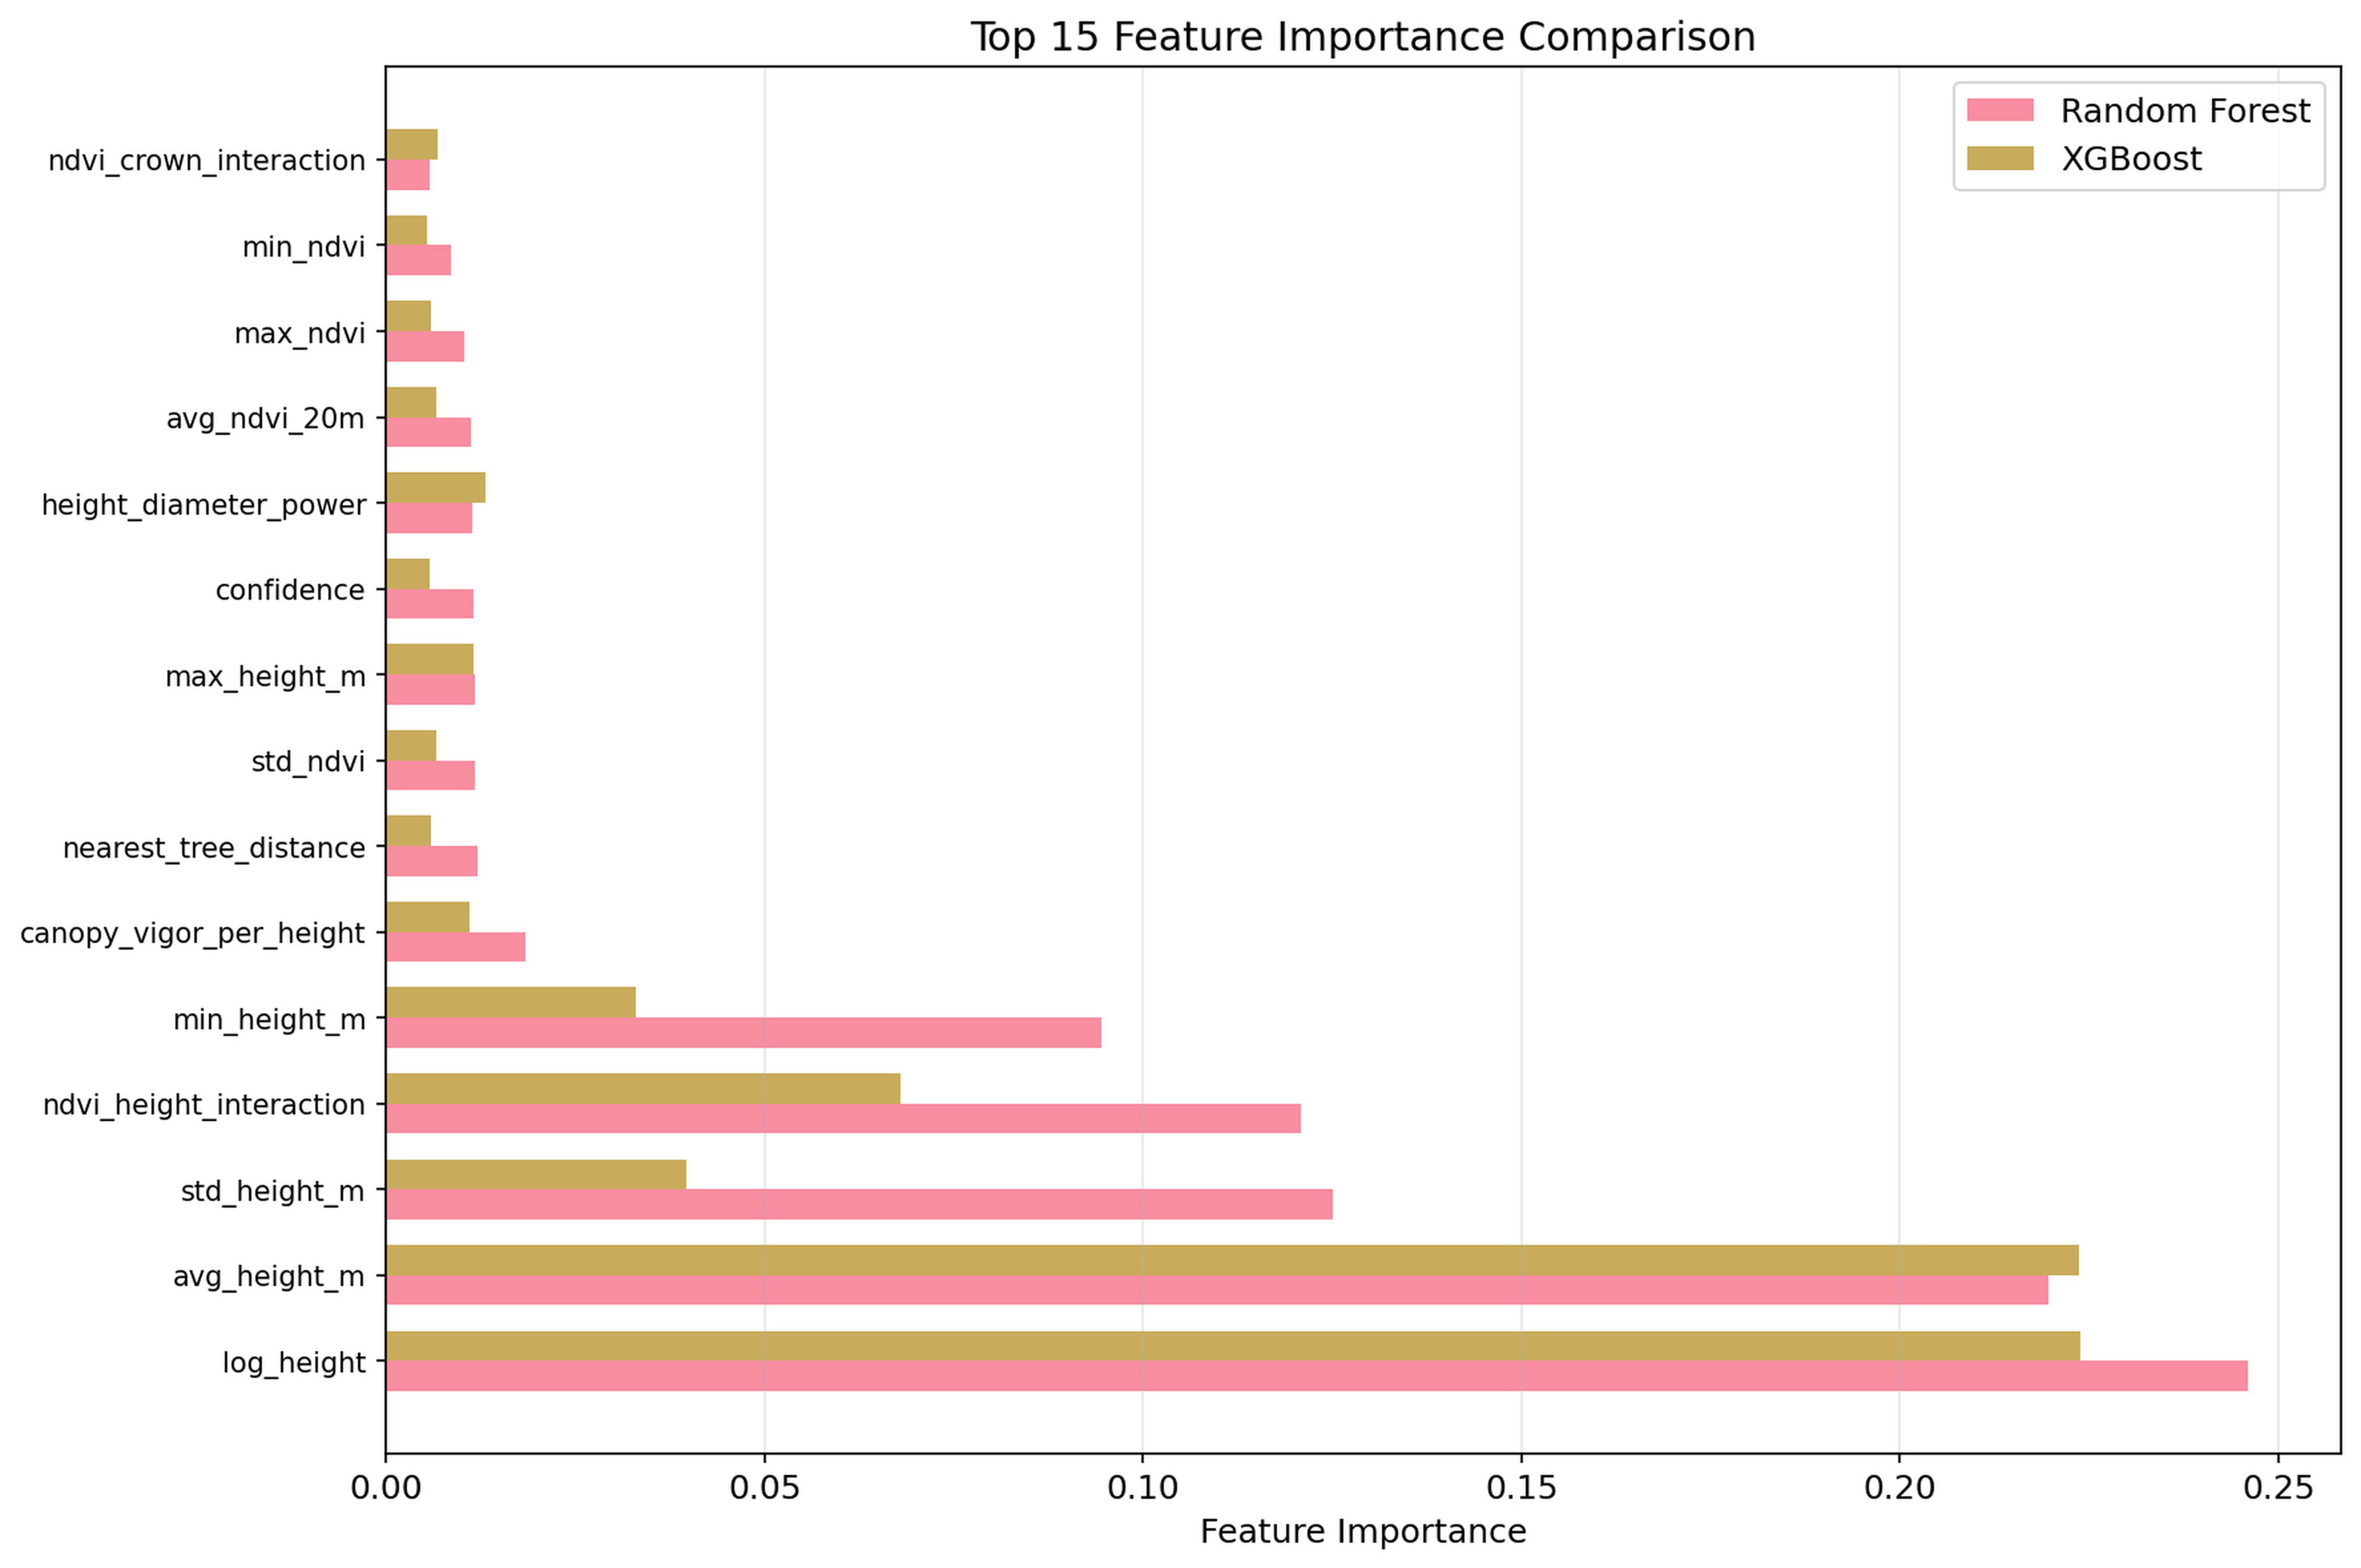
\includegraphics[width=\textwidth, height=\textheight, keepaspectratio]{figures/results/training/feature_importance_plot.png}
    \caption{Feature importance analysis for XGBoost LAI prediction model. Height-related features dominate predictions (51.3\% collective importance), with log-transformed height and average height as top predictors. NDVI-height interaction terms rank prominently, indicating spectral information modulates structural relationships.}
    \label{fig:feature_importance}
\end{figure}

Feature importance analysis revealed that tree height and its derivatives dominated model predictions (Figure 4, Table 2). The top five features collectively accounted for $59.9\%$ of total model importance, with height-related features representing $51.3\%$ when aggregated across all variants ($log_{height}$, $avg_{height_m}$, $std_{height_m}$, $min_{height_m}$, $max_{height_m}$).
Table 2. Top 15 features ranked by XGBoost importance scores.

Logarithmic height transformation ($log_{height}: 0.224$) and raw average height ($avg_{height_m}: 0.224$) exhibited nearly identical importance, confirming that vertical structure is the primary driver of LAI variation. Height category indicators (e.g., $height_{category_5-10m}$: 0.074) captured non-linear threshold effects, while height variability metrics ($std_{height_m}: 0.040$) represented crown architecture complexity.
NDVI height interaction terms ranked prominently ($ndvi_{height_{interaction}}: 0.068$, $canopy_{vigor per height}: 0.011$), indicating that spectral information modulates height-LAI relationships—likely capturing canopy density variations not explained by structure alone. Species features showed modest individual importance ($is_{deciduous}: 0.022$, $species_{group unknown}: 0.016$), collectively contributing $4.83\%$ of total feature importance across four species-related variables.
Comparison between Random Forest and XGBoost feature rankings (Figure 5) showed high concordance (Spearman's $\rho = 0.87$), with both algorithms prioritizing height features, though XGBoost assigned relatively higher importance to interaction terms and Random Forest weighted crown dimension features more heavily.

\subsubsection{Feature Category Ablation Analysis}


Systematic feature ablation quantified the marginal contribution of engineered feature categories to model performance (Table 3). This analysis directly assessed whether complex feature engineering justified the increased model complexity.
Table 3. Feature category ablation study results using XGBoost on the validation set.

%%% TO ADD Table3

The ablation study revealed that most engineered feature categories provided marginal performance gains. Removing all features beyond the base set (height, crown dimensions, NDVI) reduced $R^2$ by only $0.009$ (from $0.788$ to $0.779$), indicating that 13 fundamental features captured $98.9\%$ of achievable model performance. Individual feature categories contributed minimally: removing species features decreased $R^2$ by $0.003$, allometric features by $0.001$, and NDVI interactions by $0.003$.
The most informative configuration beyond base features was Base + Allometric ($R^2$ = $0.783$, $+0.004$ vs. Base Only), suggesting that height-diameter power relationships provided modest additional predictive power. Conversely, species information showed near-zero marginal contribution when controlling for morphology and spectral characteristics, likely because height and crown dimensions implicitly encoded species-specific architecture captured by voxel-based LAI estimation.
These findings suggest a parsimonious model using only base morphological features and NDVI would sacrifice minimal predictive accuracy ($\Delta$$R^2$ = $0.009$, $\Delta$$RMSE$ = $+0.012$) while substantially reducing feature engineering complexity and computational requirements.

\subsubsection{Species-Specific Performance Analysis}

% \begin{figure}[h!]
%     \centering
%     % Single image
%     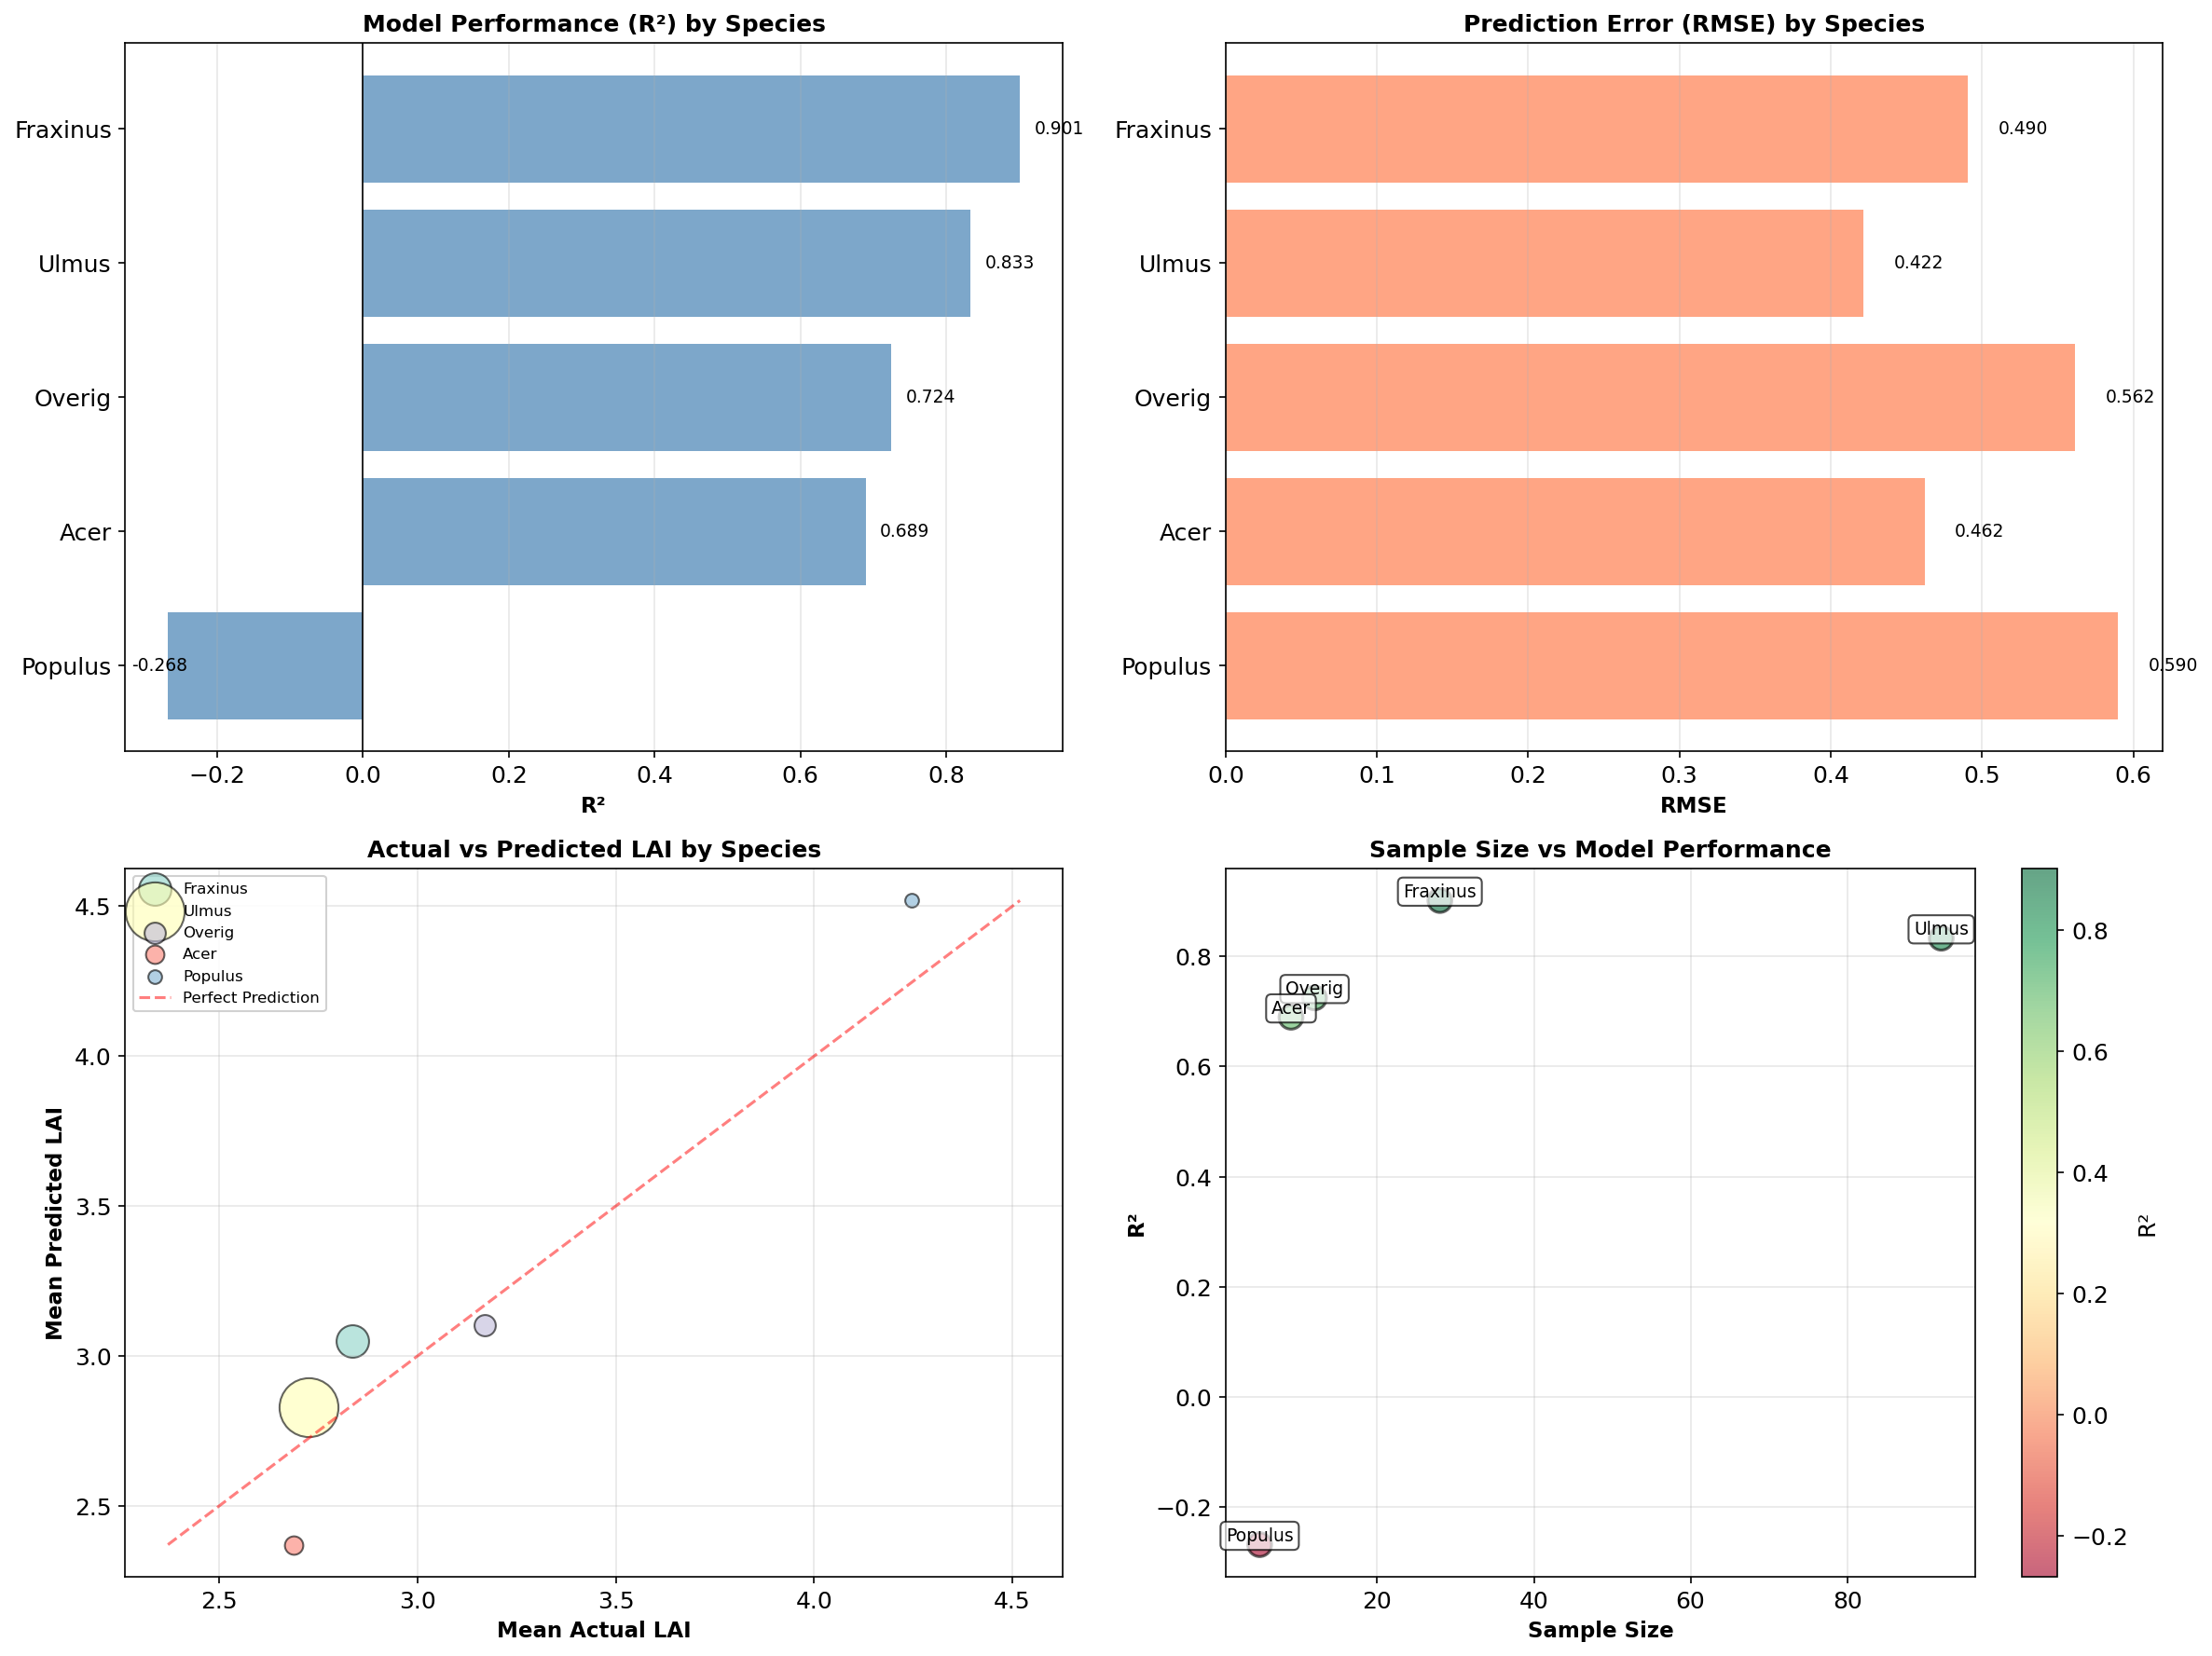
\includegraphics[width=\textwidth, height=\textheight, keepaspectratio]{figures/results/training/species_performance_analysis.png}
%     \caption{Figure 7}
%     \label{fig:species_perf}
% \end{figure}

Model performance varied substantially across species with sufficient test samples ($N \ge 20$; Figure 7, Table 4). Only species exceeding this threshold are reported to ensure statistical reliability.
Table 4. Species-specific model performance for taxa with $N \ge 20$ in test set.
Species

Fraxinus exhibited the highest prediction accuracy ($R^2$ = 0.901, RMSE = 0.490), suggesting highly consistent morphology-LAI relationships within this genus. Ulmus also showed strong performance ($R^2$ = 0.833, RMSE = 0.422) with the largest sample size (N = 92), providing the most statistically robust species-specific estimate. Acer and Quercus demonstrated moderate performance ($R^2$ = 0.762 and 0.718, respectively), though still substantially exceeding the allometric baseline.
Notably, the mixed/unknown species category (N = 412) achieved $R^2$ = 0.779—comparable to the overall test set performance—indicating that species identification is not essential for accurate LAI prediction when morphological and spectral features are available. This finding has important practical implications, as 68.2\% of trees in the full dataset lacked species labels, yet likely remain predictable using the trained model.
Performance variation across species appears partially related to LAI variance within each group: Fraxinus showed the highest $R^2$ despite moderate LAI variability (SD = 1.56), while Quercus exhibited lower $R^2$ with similar variance (SD = 1.15), suggesting that some genera maintain more consistent architectural relationships with LAI than others. Sample size effects cannot be entirely ruled out for smaller groups (Fraxinus: N = 28, Quercus: N = 23), though the monotonic relationship between sample size and $R^2$ was not observed.

\subsubsection{Ecological Relationships and Model Interpretation}

\begin{figure}[h!]
    \centering
    % First image
    \begin{subfigure}[b]{0.48\textwidth} % Adjust width as needed for spacing
        \centering
        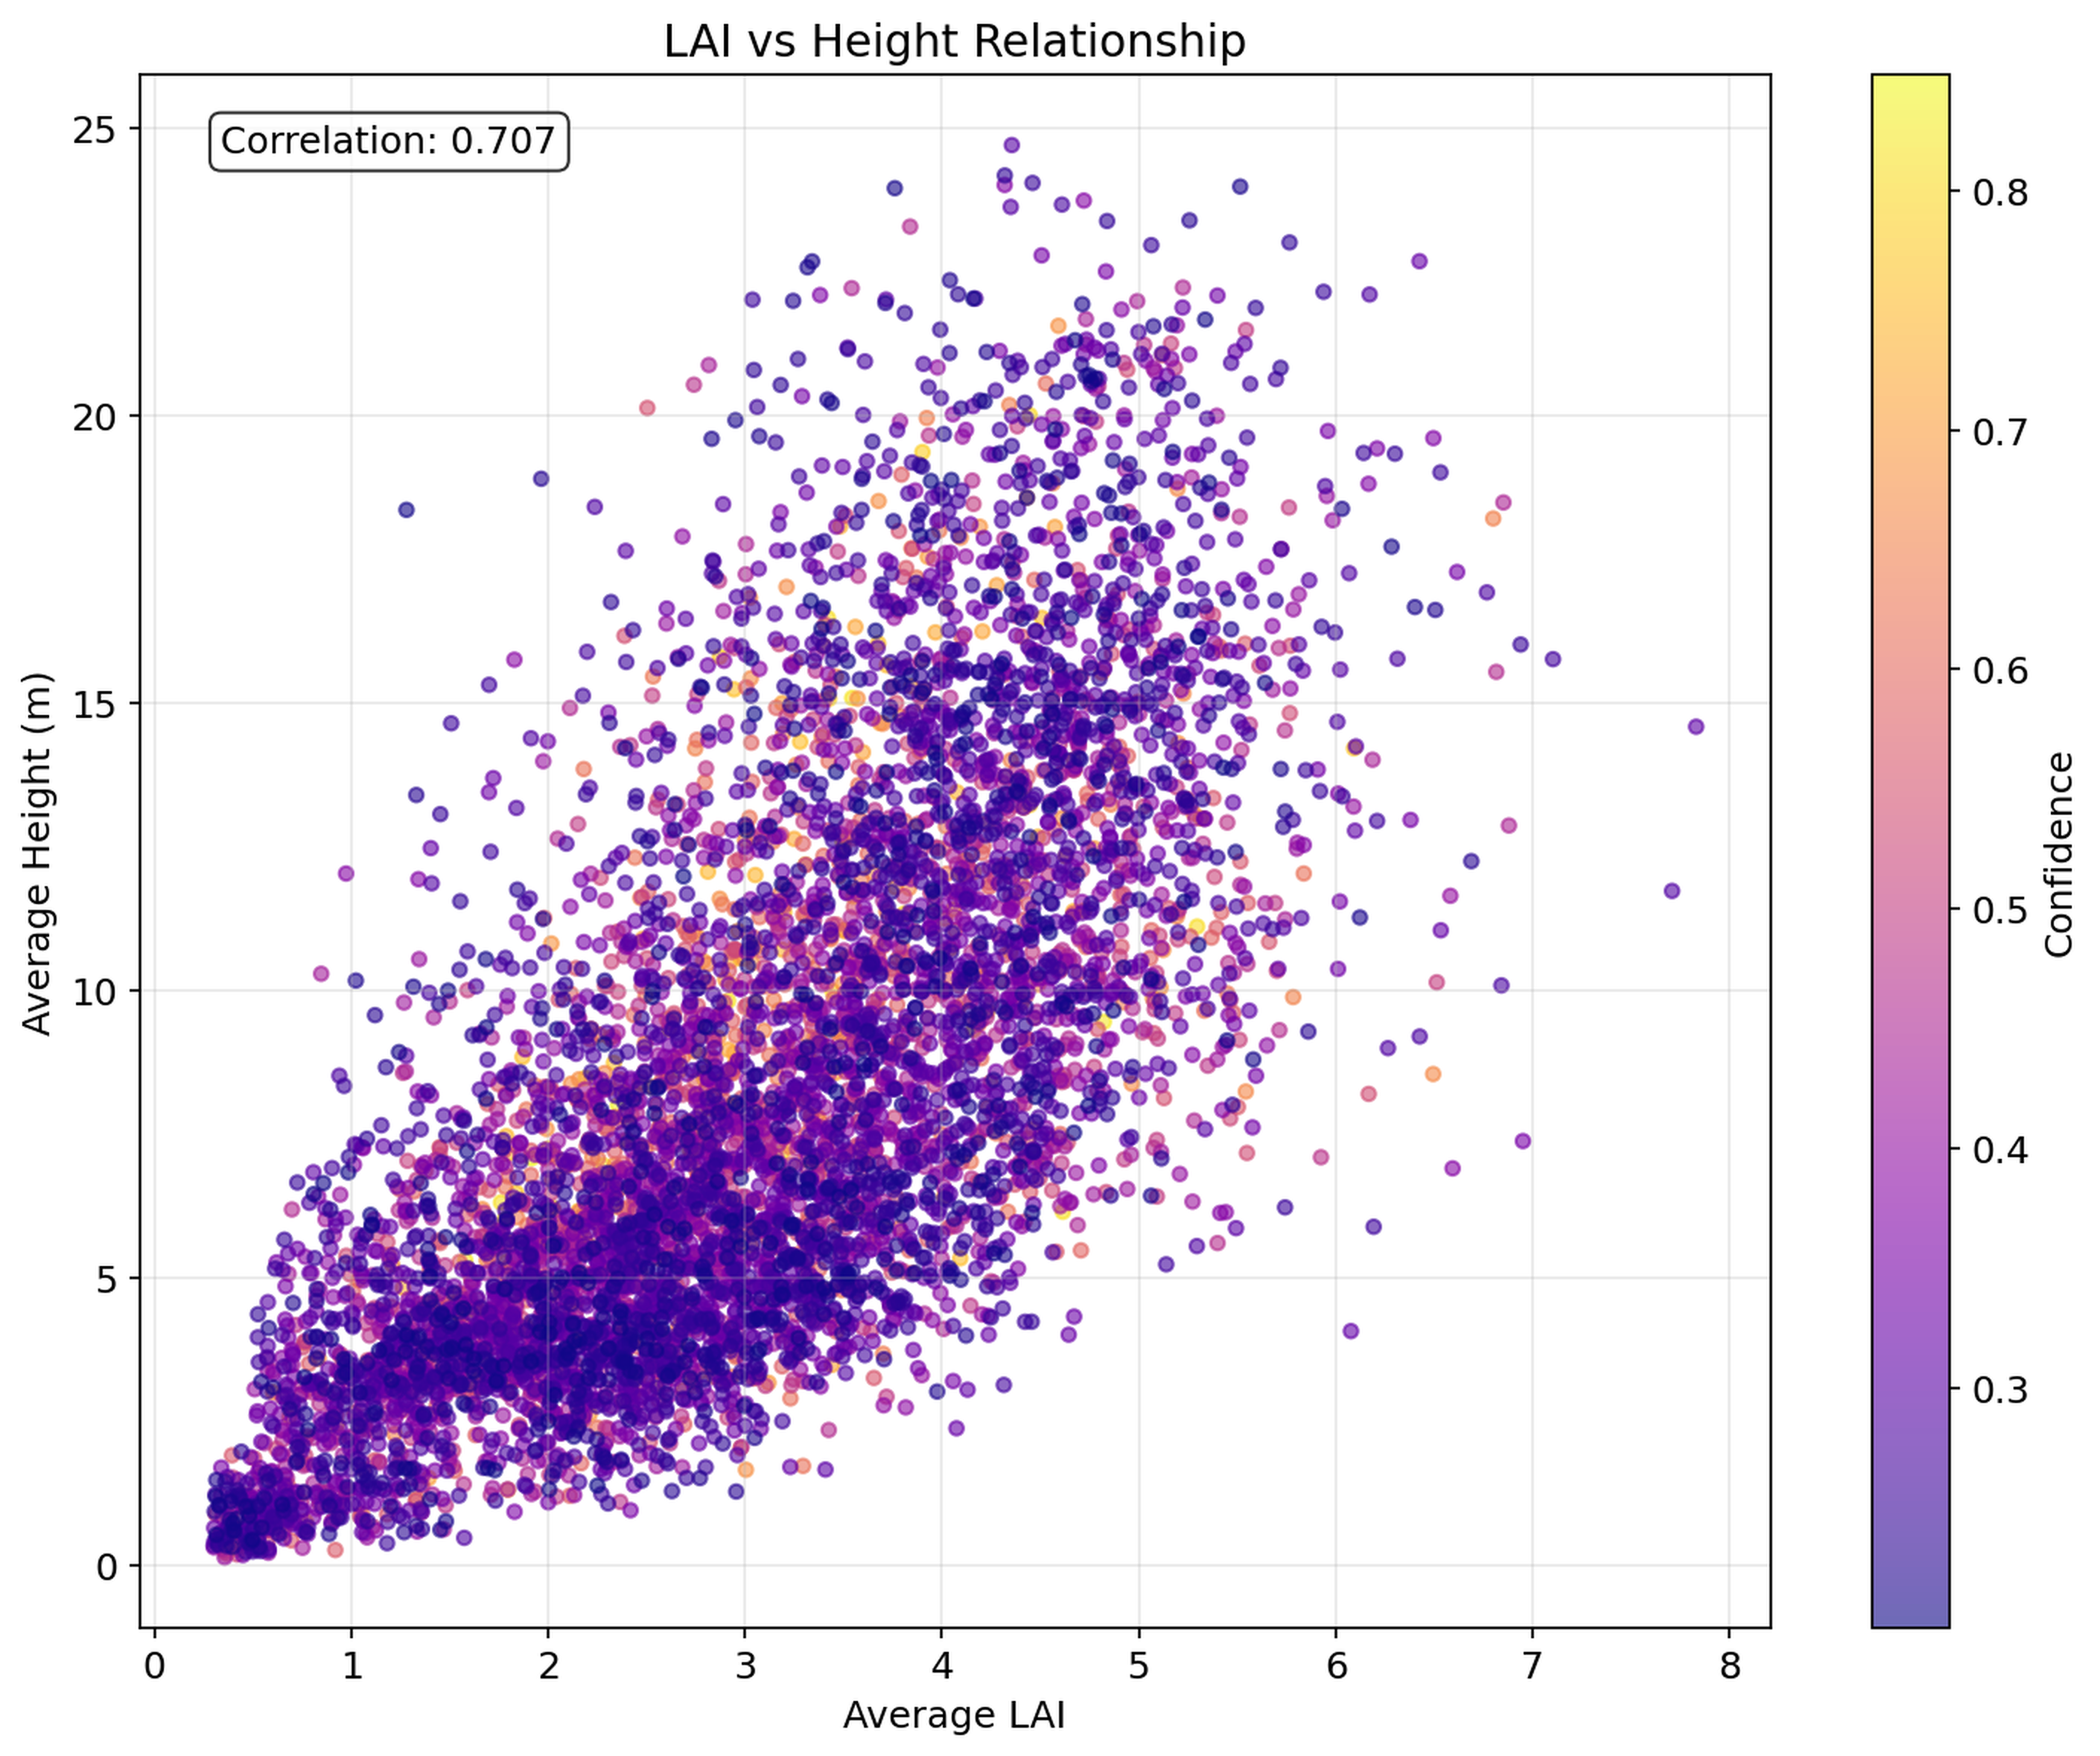
\includegraphics[width=\linewidth, height=\linewidth, keepaspectratio]{figures/results/training/lai_vs_height_analysis.png}
        \caption{LAI vs Height}
        \label{fig:lai_vs_height}
    \end{subfigure}
    \hfill % Adds horizontal space between subfigures
    % Second image
    \begin{subfigure}[b]{0.48\textwidth}
        \centering
        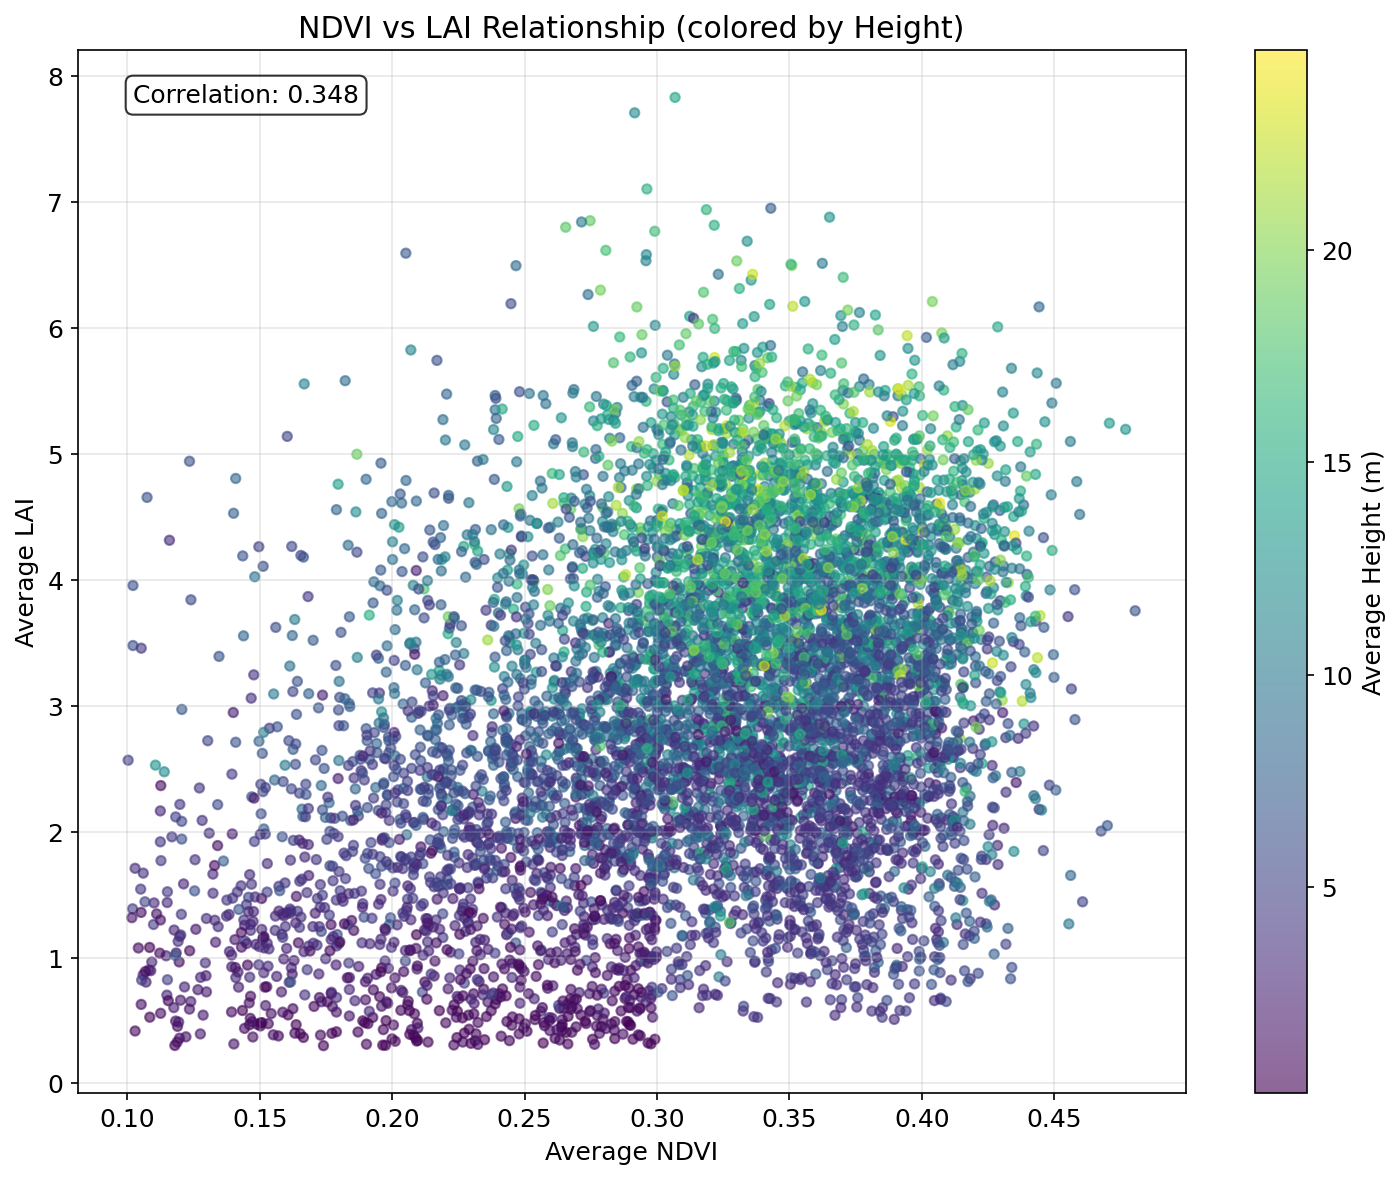
\includegraphics[width=\linewidth, height=\linewidth, keepaspectratio]{figures/results/training/ndvi_vs_lai_analysis.png}
        \caption{NDVI vs LAI}
        \label{fig:ndvi_vs_lai}
    \end{subfigure}
    \caption{Ecological Relationships}
    \label{fig:scatter_height_ndvi}
\end{figure}

Partial dependence analysis revealed interpretable ecological relationships captured by the model (Figure 8). LAI increased monotonically with tree height following a logarithmic trajectory, with rapid LAI gains from 2-10 m ($\Delta LAI \approx 2.5$ units) and gradually diminishing returns above 15 m ($\Delta LAI \approx 0.8$ from 15-30 m). This pattern aligns with known architectural constraints where vertical leaf distribution saturates as trees approach canopy closure and light limitation.
The NDVI vs LAI relationship exhibited a positive, approximately linear association ($R = 0.62$) with some saturation at high NDVI values ($>0.85$), consistent with spectral index saturation in dense canopies. Interaction effects between height and NDVI were evident: at low heights ($<8$ m), NDVI had minimal predictive power ($\Delta LAI \approx 0.3$ across NDVI range), while for tall trees ($>20$ m), NDVI variation explained substantial LAI differences ($\Delta LAI \approx 1.8$), likely reflecting canopy vigor and foliar density variations not captured by structure alone.

Crown diameter showed a weaker correlation with LAI ($R = 0.44$) compared to height, with considerable scatter, reflecting the three-dimensional nature of LAI (leaf are area per ground area) versus the two-dimensional nature of crown measurements. However, the height-to-crown-diameter ratio exhibited predictive utility (importance = 0.013), with trees showing higher ratios (narrow, tall crowns) tending toward lower LAI than broader crowns at equivalent heights.

% A Random Forest regression model was developed to predict Leaf Area Index (LAI) from tree morphological features. Hyperparameter optimization via 5-fold cross-validated randomized search identified the optimal configuration as follows: nestimators=300, minsamplessplit=20, minsamplesleaf=1, maxfeatures=0.5, and maxdepth=None. The optimized model achieved a test RMSE of 0.903, MAE of 0.685, and an R² of 0.442, indicating moderate predictive accuracy. Cross-validation results showed a mean RMSE of 0.951 with a standard deviation of ±0.081, demonstrating stable performance across data splits.

% \begin{figure}[h!]
    % \centering
    % First image
    % \begin{subfigure}[b]{0.48\textwidth} % Adjust width as needed for spacing
        % \centering
        % 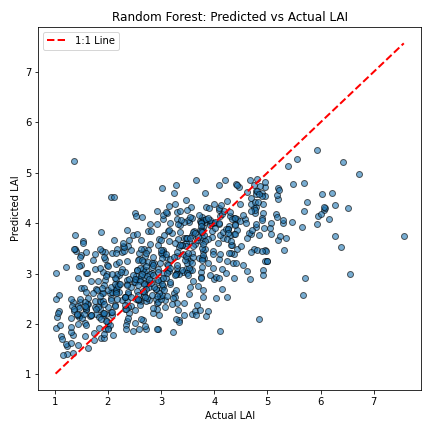
\includegraphics[width=\linewidth, height=\linewidth, keepaspectratio]{figures/results/training/pred_vs_actual.png}
        % \caption{Caption for Image 1}
        % \label{fig:image1}
    % \end{subfigure}
    % \hfill % Adds horizontal space between subfigures
    % Second image
    % \begin{subfigure}[b]{0.48\textwidth}
        % \centering
        % 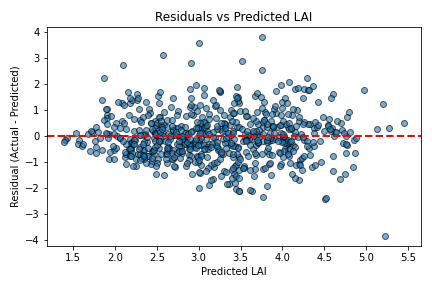
\includegraphics[width=\linewidth, height=\linewidth, keepaspectratio]{figures/results/training/residuals_vs_predicted.png}
        % \caption{Caption for Image 2}
        % \label{fig:image2}
    % \end{subfigure}
    % \caption{Two images side-by-side}
    % \label{fig:two_images}
% \end{figure}